\documentclass[11pt]{article}
\usepackage[margin=2cm]{geometry}
\usepackage{setspace}
\doublespacing
\usepackage{lineno}
\usepackage{graphicx}
\usepackage{float}
\usepackage{siunitx}


\title{
CMEE miniproject \\
\textbf{ Model selection on the abundance of freshwater microbial under the condition of global warming}}
\author{Yuxin Qin }
\date{Mar 2019}

\begin{document}
\maketitle

\begin{center}
Department of life sciences (Silwood Park)\\
Imperial College London  \\
\bigbreak
yq3018@imperial.ac.uk
\bigbreak
\bigbreak
\bigbreak
\bigbreak
\bigbreak
\bigbreak
Word Count: 2713
\end{center}


\newpage
\begin{linenumbers}
\section*{Abstract}
The increasing temperature of atmosphere has threaten the freshwater microbial communities due to the vulnerability, sensitivity and dependancy to temperatue of the freshwater systems.
Reduced bodysize is an obvious biological response to the warming condition in many ectothermic taxa for warming significant affects the life history and metabolic mechanism.
Yvon and Stewart conducted similar mesocosm experiments to test the impact of warming condition on freshwater microbial communities, while they came to different conclusions.
Yvon claimed that community biomass declined consideratly under warming condition showing that the slope of log(abundance) against log(bodysize) in warming condition was steeper.
However, Stewart's experiment came to an inconsistent conclusion which cannot prove the statement of Yvon.
The aim of this article was to carry out the model selection by reanalyzing Stewart's data and comparing the allometric scaling model and to Plante-Downing model.
It turned out that the Plante-Downing model performed better than the allometric scaling model in Akaike information criterion (AIC), while the allometric scaling model provided us valuable information on understanding the impacts of global warming on freshwater microbial communities.


\section*{Introduction}
According to the IPCC report published in 2018, the surface temperature of the earth has increased approximately \SI{1.0}{\celsius} compared to pre-industrial levels and it tends to reach \SI{1.5}{\celsius} between 2030 and 2052 if global warming continues at current rate in the following years \cite{IPCC}.
Since the phrase global warming first appeared in 1957, many scientists have studied the impacts of global warming in different scales and different organisms such as climate change, crop production, coral bleach and so on \cite{weart2009discovery}.
Due to temperature dependency and the long-term exposure to environmental stressors and the vulnerability of the freshwater system, it is significant to study the impacts of global warming on it \cite{arnell1996effects}.
The previous study of global warming on freshwater system mainly focuesed on the distribution of freshwater and the potential changes of freshwater fishes \cite{carpenter1992global},
while many recent studies discovered that warming has obvious impacts on freshwater microbial communities by means of mesocosm experiments. \\
Utilizing mesocosm experiments to examine the impacts of warming on freshwater microbial communities allows researchers to control temperature, a key factor, between the experimental group and the control group.
Mesocosm experiments also provide freshwater microbial communities less differences to the real natural environment compared to other ordinary laboratory experiments. By means of mesocosm expeiments, Yvon discovered that warming significantly reduced the total biomass of freshwater microbial community and increased the gradient steepness of community size spectrum \cite{yvon2011warming}.
Rebeca Stewart from the University of London carried out a similar mesocosm experiment as Yvon did during her PhD, whereas with a different conclusion. She claimed a contrary opinion that warming has not shown a significant impact on freshwater microbial community biomass and increased gradient steepness of the community size spectrum \cite{rebecca}.
In order to prove the actual influences of warming on freshwater microbial communities, a reanalysis of Stewart's data has been carried out in this study. \\
Stewart's mesocosm experiment consisted of 2 groups of ponds, the control group and the experiment group. Each group contained 10 artificial outdoor ponds with the capacity of approximately \( 1 m^3\) water.
The water temperature in experiment ponds were being maintained between 3-5 \SI{1.0}{\celsius} by electronic heating elements.
All the experiment ponds and the control ponds were arranged randomly by the block design.
The biota seeded in the mesocosms were from the river Frome, Dorset, UK, containing 5 main groups of microbes, ciliate, algae, meiofauna, flagellate and heterothrophic protists.
These microbes were seeded to the ponds 10 months prior to experiments for required natural colonisation. The sample of microbial communities was performed monthly from February 2009 to January 2010.
10 ml water samples collected from each pond using a sterile syringe at three depths of the pond, the water surface, the middle water column and the sediment surface respectively.
Afterwards, 1 ml subsample was removed from each 10 ml water sample to a 1 ml Sedgwich-Rafter counting cell for further analysis using light microscopy.
Stewart identified the group, family, genus, species and feeding type of each microbial subsample and recorded the shapes lively under microscopy.
The length and width of each microbial individual containing in the 1 ml subsample have been measured by image analysis software ImageJ and Q capture.
Therefore, the biovolume, abundance and biomass of each species or groups were generated from the original data. \\
The objective of this article is to analyze the relationship among abundance, bodymass and biomass in freshwater microbial communities under warming condition.
Shrinking bodysize has been observed as a severe ecological response to climate change in a wide range of ectothermic taxa \cite{walters2006temperature}.
Bodysize is regarded as a fundamental ecological feature of many biological characteristics such as reproduction, population density and growth rate, which are in an allometric scaliing relationship with bodysize \cite{peters1983effect}.
The allometric scaling of bodysize and biological characteristic are a general criteria applied in many systems including freshwater system \cite{yvon2011warming}.
Another model, Plante-Downing model, is an empirical model with the merit of prediction for the invertebrate population in freshwater system\cite{plante1989production}.
This model selection research intended to do the data fitting of freshwater microbial collected by Stewart, with the coincidence evaluation of the two above models by means of Akaike information criterion (AIC).

\section*{Methods}
\section*{1 Data handling}
The data selected in this article are based on the thesis of Rebecca Stewart.
Some suspectable mistakes have been observed in the original datasheet, and for the sake of well-suited candidate model to the analysis, filtered blank space in temperature have been refilled, abnormal data have been deleted, the biovolume, bodymass and biomass have been recalculated in each data recorded.
Biovolume of each freshwater microbial was calculated in length and width measured by the microscope according to the shape recorded, and equations applied to calculate the biovolume were followed the paper of Hillerbrand's paper\cite{hillebrand1999biovolume}.
Bodymass referring to the individual mass, calculated by the equation $Bodymass = Biovolume * 0.14 * 1.1 $ according to Julia Resis's paper \cite{reiss2008existing}.
Biomass referring to the carbon dry mass of freshwater taxa, was calculated by the mutiplication of 0.25 bodymass and abundance.
Therefore, these convenient recognized data for the fitting models have been obtained.

\section*{2 Fitting model}
Two models, the allometric scaling model and the Plante-Downing model, have been introduced in this study to fit the abundance and bodymass values. The result coincidence of these two models has been compared on accounts of Akaike information criterion (AIC).    \\
\textbf{2.1 Allometric scaling model} \\
The allometric scaling model is shown below, where $y$ is the characteristic of interest, $x$ is bodysize. $a$ and $b$ here are constants.
The constant $a$ can be considered as the ratio of specific growth rate between $y$ and $x$ \cite{huxley1950relative}.
For the sake of better fitting, the abundance was assumed as the biological characteristic $y$ and the bodymass as the individual bodysize $x$.
The logarithm operation applied on both bodymass and abundance, afterwards, the gradient of this linear model indicates the growth rate of bodymass and abundance.
The slope of this linear model can indicate the growth rate of bodymass and abundance.
\begin{equation}
     y= b x^a
\end{equation}
\textbf{2.2 Plante-Downing model} \\
The Plante-Downing model is an empirical model shown below, where $P$ is the population of freshwater invertebrate, $\overline{B}$ is the annual mean population biomass, $\mathit{W}_{m}$ is the maximum individual bodymass and $T$ is the ambient surface temperature \cite{plante1989production}.
This model has been proved to fit freshwater invetebrate communities annually quite well.  \cite{plante1989production}.
In the circumstance of this study, the model has been fitted in monthly span and replaced $P$ in the original formula with abundance. The rest parameters were performed as the original ones.
\begin{equation}
     \log(P) = a +b \log(\overline{B}) - c \log(\mathit{W}_{m}) + d T
\end{equation}
\textbf{2.3 Model selection} \\
In terms of model selection methods used in publications, AIC and BIC (Bayesian information criterion) are the most popular methods showing that AIC accounts for 84\% of all and BIC accounts for 14\% \cite{aho2014model}. AIC utilized the Kullback-Leibler information lost to measure the discrepancy between the true model and the approximating model \cite{wagenmakers2004aic}. BIC also called the Schwarz or SIC criterion. The major difference between AIC and BIC is that AIC can better simulate situations with a true model, but BIC fits the situations maninly based on a true model \cite{aho2014model}. \\
The AIC has been chosen as the criterion for comparison of these two models since the relationship of abundance and bodymass in freshwater microbial did not reveal by a true model but only one model using bodymass to predict the abundance of freshwater.
The calculation of AIC was based on the Johnson's papaer \cite{johnson2004model}.
The normal AIC applied to this study because neither the number of the free parameters $p$ in two selected models exceeded $n/40$ (n is the sample size). The sample size is 4271,  $n/40 =4271/40 = 106.67 $, and the number of free parameters in the allometric model is 2 and the number of free parameters in Plante-Downing model is 4, thus obviously, both 2 and 4 are smaller than the 106.67. Hence, the second order deriative of AIC, the $\mathit{AIC}_{c}$, was not necessarily to apply in this paper since it is normally used to correct small sample size. \\
The formula to calculate AIC is shown below. In this formula, $L(\hat{\theta}|y)$ is the likelihood of the model parameters given by the data. For models fitted by least squares with the usual assumptions,
$L(\hat{\theta}|y)=-n/2\ln(RSS/n)$. RSS here is the residual sum of squares for a linear model and n is the sample size. $p$ is the free parameter of the tested model.
\begin{equation}
AIC = -2 \ln [ L (\hat{\theta}|y)] + 2 p = -2 \ln [-n/2\ln(RSS/n)] + 2 p
\end{equation}

\section*{3 Computing languages}
The major computing languages programmed in the miniproject are bash, Python and R. Bash was used to running the workflow as creating the report in LaTeX,running Python scripts and R scripts. The calculation, model fitting and plotting are all performed in R version 3.2.3 (2015-12-10). The model fittings in this article have been done by lm in R, and the plots were produced by ggplot2 basically. Functions have been created to generate the coefficient table and AIC table automatically in R. Thress reasons for selected R to do calculation, model fiting and plotting: at first, the size of raw data only occupied 7.4Mb which is proper for R; the calculation and model fitting in this miniproject are simple and are able to be handled by R efficiently; at last, R provides a better visualization than Python.
As for the ANOVA analysis in the article, python 3.7 has been performed on account of the lack of P value in ANOVA analysis when using lmer to do ANOVA in R is more complex than using statsmodels in Python. \\

\section*{Results}
\section*{1 Community biomass}
According to Figure 1, it is obvious that the mean community biomass under warming condition is smaller than that of the cold or ambient condition. The ANOVA analysis shown in Table 1 has shown that the treatment and month both have considerable effects on community biomass. It can be concluded that the biomass of freshwater microbial community largely reduced under warming conditions.
\begin{figure}[H]
  \centering
  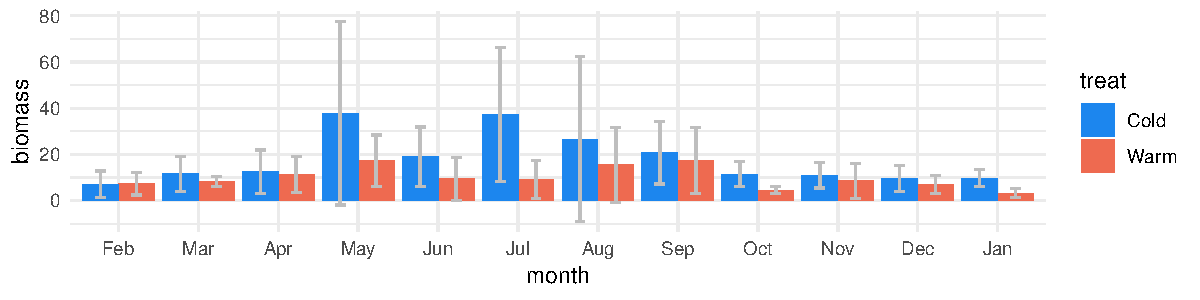
\includegraphics[scale = 0.8]{../Graph/CommunityBiomassPlot.pdf}
  \caption{\textbf{The mean community biomass in each month.}  }
\end{figure}

\begin{table}[H]
  \centering
  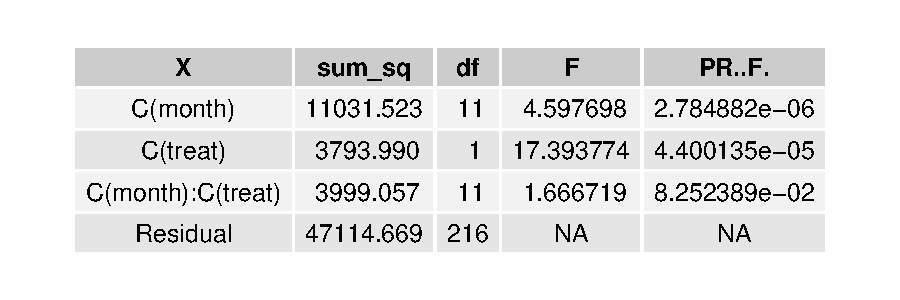
\includegraphics[scale = 0.8]{../Graph/anova.pdf}
  \caption{\textbf{The ANOVA analysis of community biomass}  }
\end{table}

\section*{2 Allometric scaling model}
The coefficients of the allometric scaling model under different conditions were listed in Table 2.
By plotting the slope of warming condition and ambient condition on the same graph as shown in Figure 2, it is predictable that the slope of the ambient condition is higher than the warming condition except for February, the first experiment month.
The slope of the linear model is also the coefficient of $log(bodymass)$, indicating a higher growth rate in population in the ambient condition compared to warming condition, which supports the conclusion driven by Yvon.
The bodysize of ectothermic taxa mainly determined by two ecological factors, nutrient supply and metabolic rate \cite{sheridan2011shrinking}. Since the nutrient supply is the same among all mesocosm ponds, the reduction of bodymass in warming condition is attributed to the decreasing metabolic rate. Figure 2 implicated that one potential consequence of rising temperature is the decline of the metabolic rate of freshwater microbial communities.  \\
By applying linear regression on the allometric scaling model show in Figure 3 and comparison of observed value against the predicted value of $log(abundance)$ shown in Figure 4, it is apparent the data did not express good fit into the model.

\begin{table}[H]
  \centering
  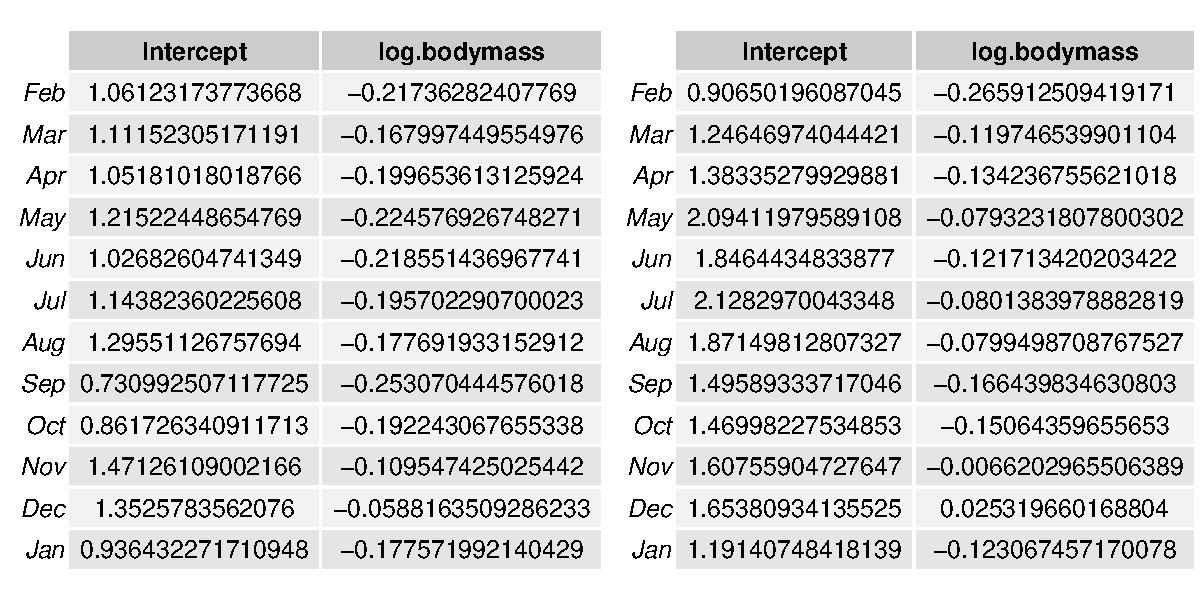
\includegraphics[scale = 0.8]{../Graph/ascoef.pdf}
  \caption{\textbf{The coefficients of the allometric scaling model.}  The table on the left is the coefficients under warming condition. The table on the right is the coefficients under ambient condition. }
\end{table}

\begin{figure}[H]
  \centering
  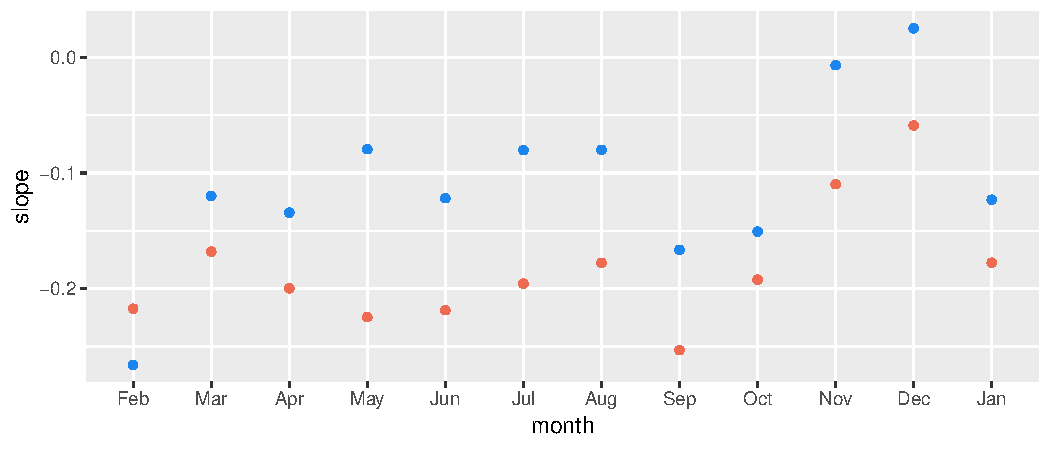
\includegraphics[scale = 0.8]{../Graph/ascoefplot.pdf}
  \caption{\textbf{The slope of allometric scaling model in each month.}  The red dots represents samples of warming condition and the blue dots represents samples of ambient condition. }
\end{figure}

\begin{figure}[H]
  \centering
  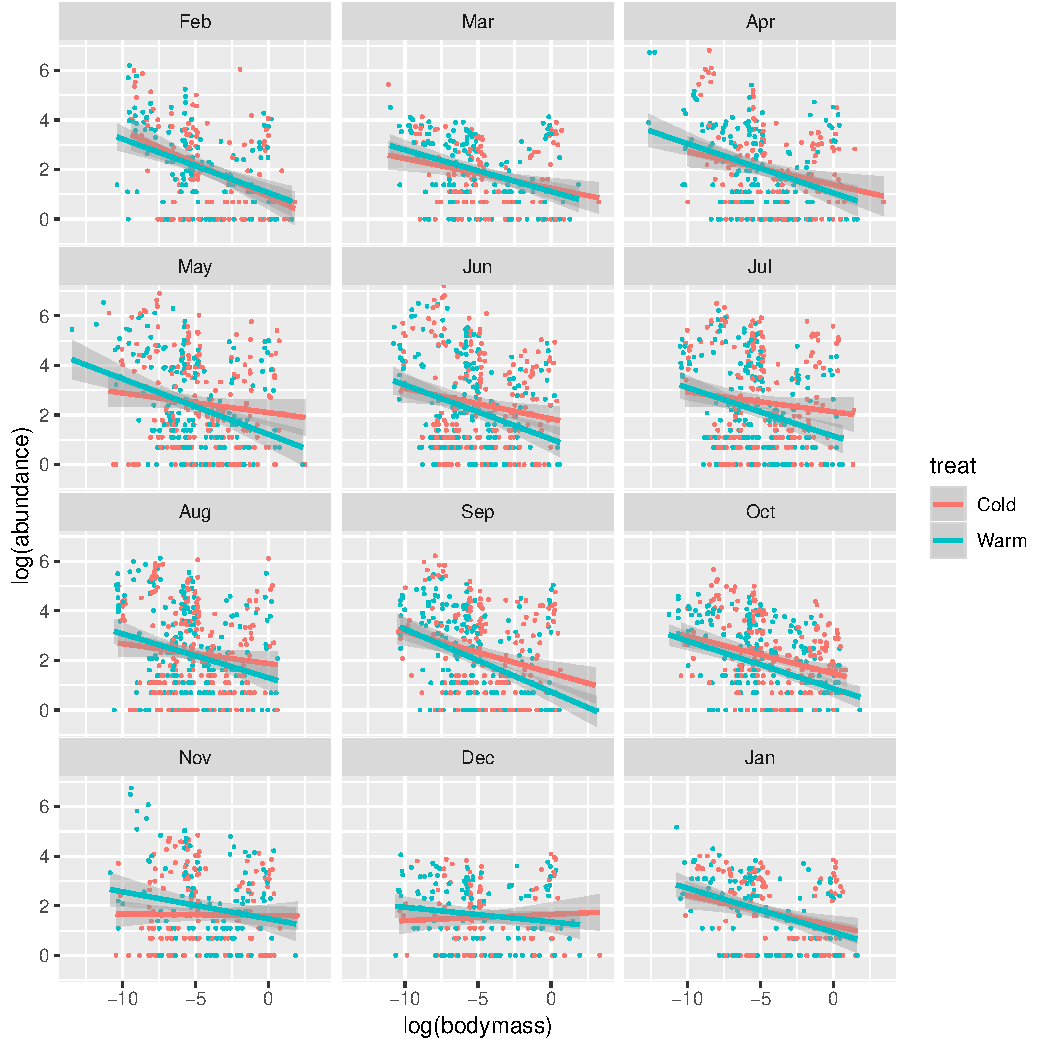
\includegraphics{../Graph/as12l.pdf}
  \caption{\textbf{Linear regression graph of the allometric scaling model.}
  Red scatters in the graph represent samples of warming condition and the blue scatters represent samples of ambient condition. }
\end{figure}

\begin{figure}[H]
  \centering
  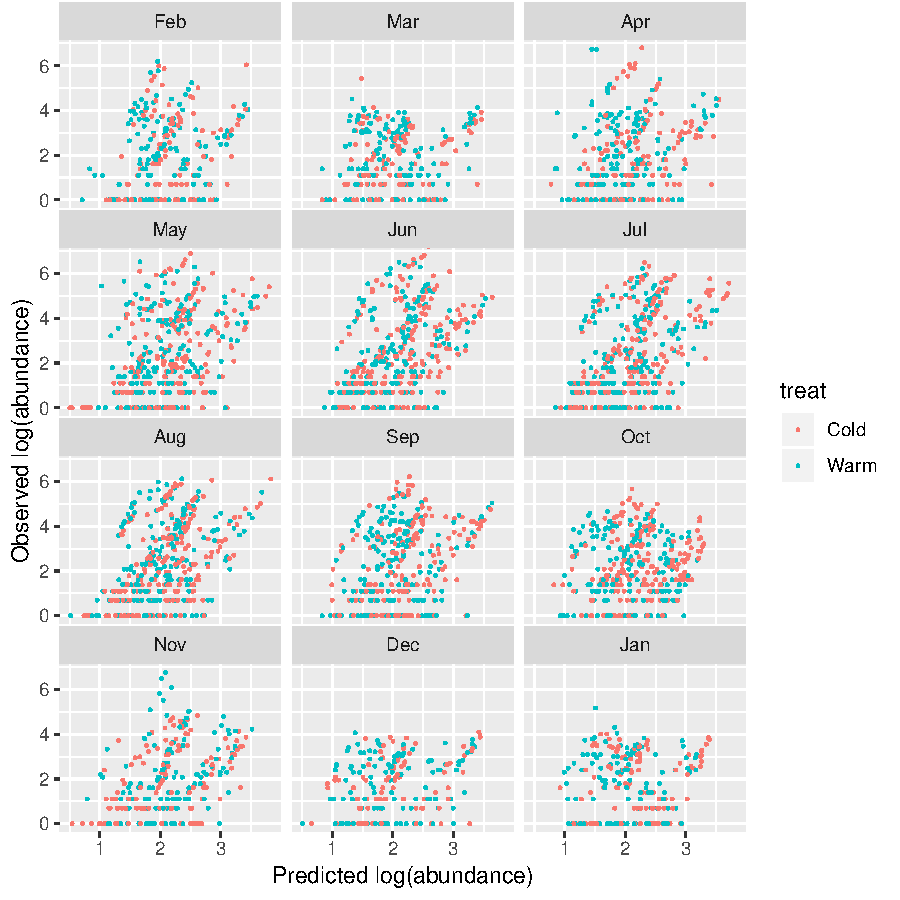
\includegraphics[scale = 1.2]{../Graph/as12op.pdf}
  \caption{\textbf{The observed value and predicted value of
  the allometric scaling model.}
  The red points in graph represent samples of warming condition and the blue points represent samples of ambient condition. }
\end{figure}

\section*{3 Plante-Downing model}
The coefficients in Plante-Downing model of different conditions were listed in Table 3. According to the plotting of the observed value against predicted value of $log(abundance)$ as shown in Figure 5, Plante-Downing model fitted expectedly well into the model.



\begin{table}[H]
  \centering
  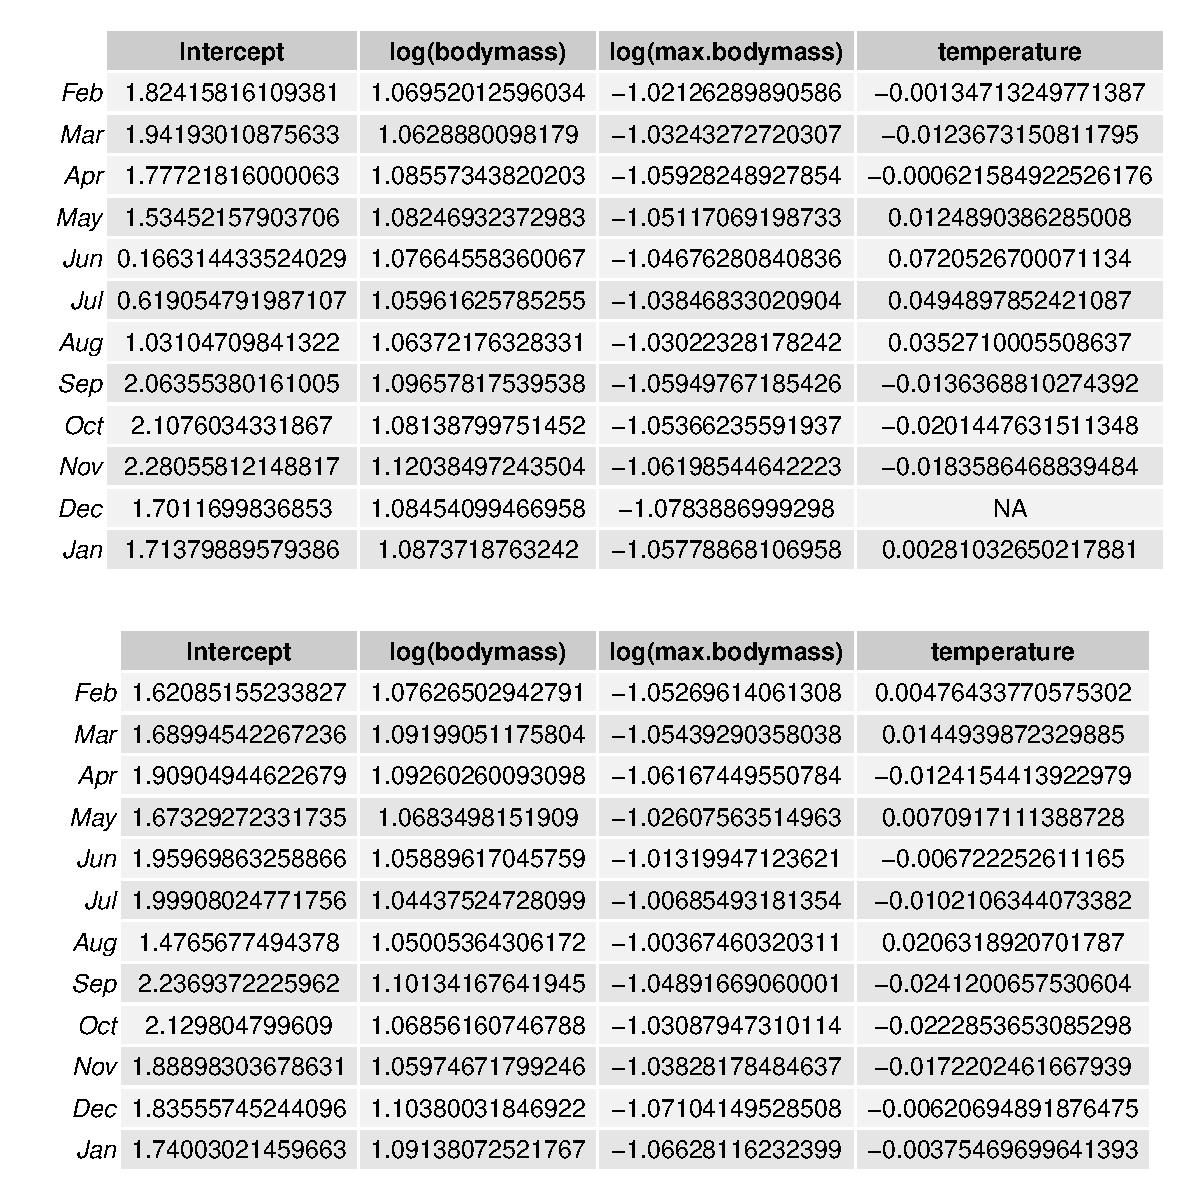
\includegraphics[scale = 0.7]{../Graph/pdcoef.pdf}
  \caption{\textbf{The coefficients of the Plante-Downing model.}
   The upper table  is the coefficients under warming condition. The lower table is the coefficients under ambient condition. }
\end{table}

\begin{figure}[H]
  \centering
  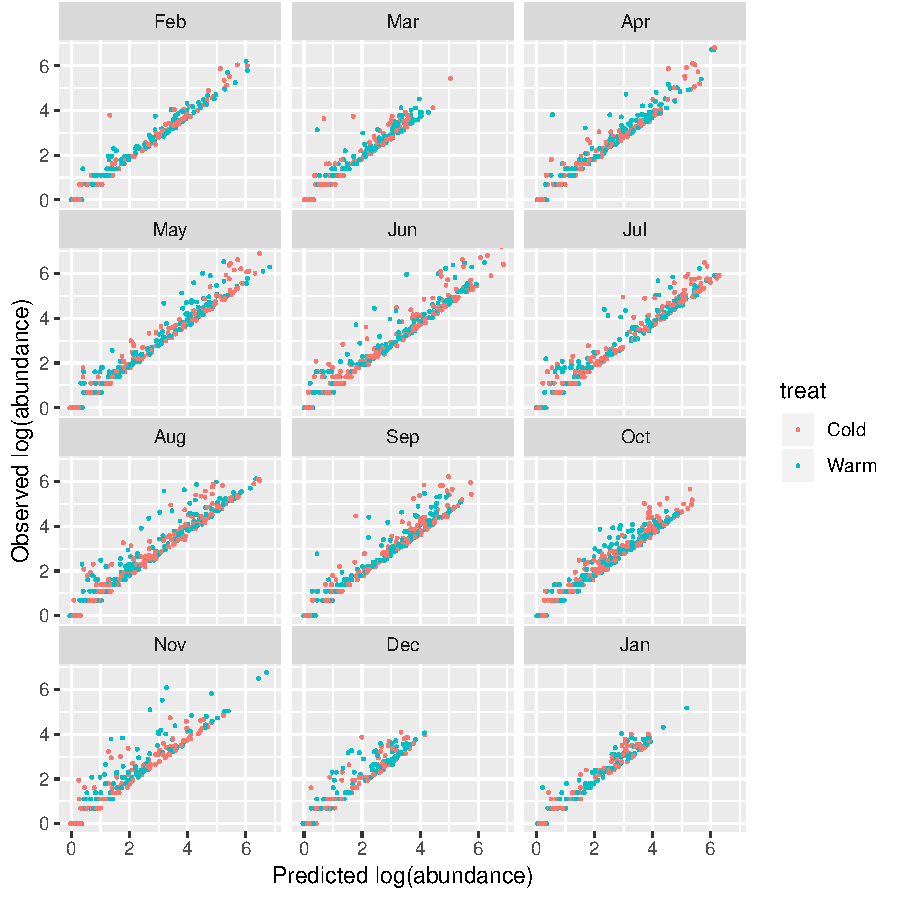
\includegraphics[scale= 1.2]{../Graph/pd12l.pdf}
  \caption{\textbf{The observed value and predicted value of
  the Plante-Downing model.}
  The red dots in graph represent samples of warming condition and the blue dots represent samples of ambient condition. }
\end{figure}


\section*{4 Model selection}
Generally, models with relatively low AIC are regareded as better-fitted models. Based on the AIC results of both models shown in Table 4, it is clear that Plante-Downing model is a better model to explain the interrelations between abundance and bodymass of freshwater microbial communities.


\begin{table}[H]
  \centering
  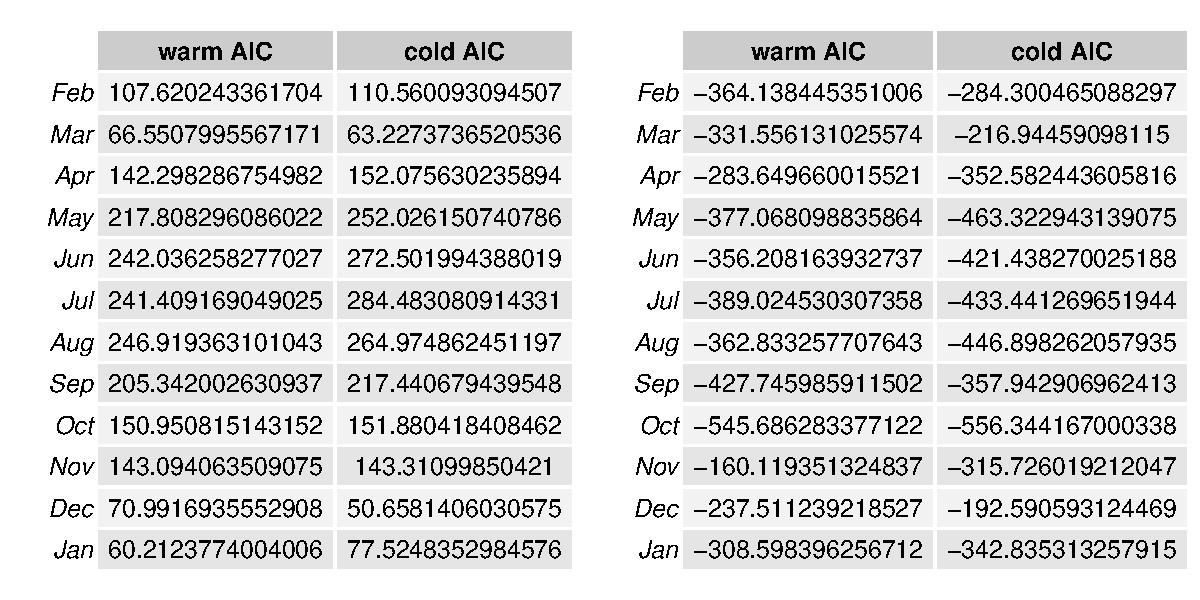
\includegraphics[scale = 0.8]{../Graph/aic.pdf}
  \caption{\textbf{The AIC value of the two model under both warming and ambient condition.}
  The table on the left is the AIC value of the allometric scaling model.The table on the right is the AIC value of Plante-Downing model. }
\end{table}

\section*{Discussion}
From the above analysis, it is clearly concluded that Plante-Downing model is the better choice for freshwater microbial communities data analysis than the allometric scaling model as it showed a more firm scatterplot fitting, while the widely used allometric scaling model still provided us with a reference and some feedback.
The lack of performance of allometric scaling model in AIC largely attributed to the small abundance in many sampled species.
It could be observed in Figure 3 that a certain amount of scattering points lying on the line $y= 0$, indicated that the abundance value of these sampled species in that month is 1. \\
Although the Plante-Downing model revealed a good performance in AIC, it is necessary to realize that this empirical model was very likely to have a good fit for the data in this case as the biomass here was calculated by the multiplication of bodymass and abundance.
Assuming $A$ as abundance and $B$ as bodymass, subsituting $\overline{B}$ with ${B}_{mean}*A$ into the formula 2, then we can discover that $ \log(A) = a +b \log({B}_{mean}*A) - c \log(\mathit{B}_{max}) + d T$.
This formula can be transformed to $\log(A) = \log(({B}_{mean}*A)^b/\log(\mathit{B}_{max})^c) + d T + a$.
Due to the appearance of abundance on both sides of the equation, the model is available to perform a great fit by adjustment of constant values b and c.
For further optimizing the Plante-Downing model of this case, it is better to use projection to calculate the population of freshwater microbial communities in the following months, and then the abundance of each month are able to link sequentially.  \\
In addition, the exclusion of some abnormal data might affect the model fitting results. Those abnormal data have been deleted because the microbial individuals were recorded as spherical shape whereas the length and width recorded was quite different.
For example, the length and width of taxa recorded having a spherical shape is 1200 $\mu m$ and 21 $\mu m$. The total number of data deletion was 313 and it is necessary to remain the doubts of unknown influences to the model fitting results.
Thoses deleted individuals might play important roles in the freshwater microbial communities such as a predator. For further detail studies, it is preferable to implement advanced data analysis algorithms rather than simply omitting these abnormal data.

\section*{Conclusion}
In conclusion, the Plante-Downing model performed better than the allometric scaling model in terms of AIC. The results of this article supported Yvon's statement that freshwater microbial communities biomass decreases in warming condition. This study also validated Yvon's statement that the gradient of linear litting in warming condition was steeper, implicating freshwater microbial communities at a relatively lower growth rate of abundance under warming condition.



\newpage

\bibliographystyle{plain}
\bibliography{minbib.bib}

\end{linenumbers}

\end{document}